\documentclass[12pt,a4paper]{article}

\usepackage{preamble}

\addbibresource{refs.bib}

\begin{document}

\pagenumbering{Alph}  % Numeración alfabética para titlepage (evita duplicados)
\begin{titlepage}
	\vspace*{-2cm}
	% --- LOGOTIPOS (ALINEADOS ARRIBA, IZQUIERDA Y DERECHA) ---
	\noindent
	
\includegraphics[width=0.35\textwidth]{ule.jpg}
	\hfill
	
\includegraphics[height=2.5cm]{escudo-ingenierias.png}

	\vspace{0.2cm}

	% --- CUADRO AZUL PARA EL TÍTULO ---
	\begin{tcolorbox}[colback=maincolor,colframe=maincolor,arc=0pt,outer arc=0pt,grow to left by=3cm,grow to right by=3cm,fontupper=\color{white}]
		\centering
		\vspace{0.8cm}
		{\Huge \bfseries INSTALACIONES II}\\[0.4cm]
		{\Large \titulo}
		\vspace{0.8cm}
	\end{tcolorbox}

	\vspace{0.5cm}
	\begin{center}
		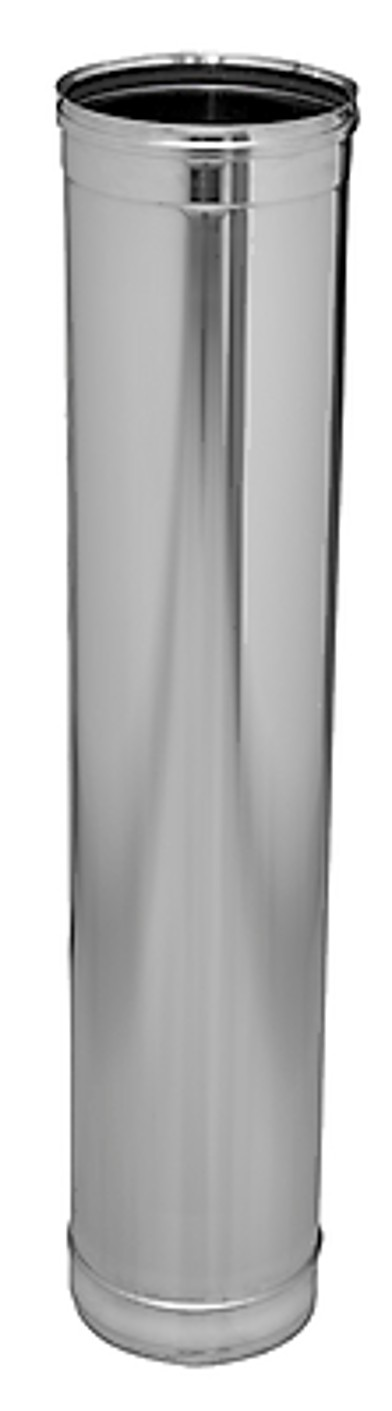
\includegraphics[height=9cm, keepaspectratio]{Figuras/chimenea_recta.jpg}
	\end{center}
	\vfill

	% --- AUTORES Y DATOS (ALINEADOS A LA DERECHA, SIN CUADRO) ---
	\begin{flushright}
		\large
		\begin{tabular}{@{}ll}
			\textbf{Grupo:}   & 1 \\ [5pt]
			\textbf{Autores:} & Alberto España Carrete   \\
                        & Carlos Fernández Palanca \\
                        & Rubén Modino López      \\
                        & Juan Diego Niño González \\ [5pt]
      		\textbf{Tutor:}   & José Luis Falagán Cavero
			
		\end{tabular}
	\end{flushright}

	\vspace{0.5cm}

	\begin{center}
    {\fontsize{16pt}{19pt}\LARGE(Mayo, 2026)}
  	\end{center}
\end{titlepage}

\pagenumbering{roman}
\clearpage
\pagestyle{empty}

{
	\hypersetup{linkcolor=black}
	\tableofcontents
	\clearpage

	% --- Índice de figuras ---
	{
		\let\oldnumberline\numberline
		\renewcommand{\numberline}{\figurename~\oldnumberline}
		\listoffigures
		\phantomsection
		\addtocontents{toc}{\protect\cftpagenumbersoff{section}}
		\addcontentsline{toc}{section}{\listfigurename}
		\addtocontents{toc}{\protect\cftpagenumberson{section}}
	}
	\clearpage

	% --- Índice de tablas ---
	{
		\let\oldnumberline\numberline
		\renewcommand{\numberline}{\tablename~\oldnumberline}
		\listoftables
		\phantomsection
		\addtocontents{toc}{\protect\cftpagenumbersoff{section}}
		\addcontentsline{toc}{section}{\listtablename}
		\addtocontents{toc}{\protect\cftpagenumberson{section}}
	}

}

\pagenumbering{arabic}
\pagestyle{contenido}
\section*{Resumen}
\phantomsection
\addcontentsline{toc}{section}{Resumen}

La presente práctica desarrolla el modelado, cálculo y optimización de una instalación receptora de gas natural para un edificio de viviendas mediante DMElect/GASCOMB. El trabajo parte de una acometida en Media Presión A (MPA), de las potencias nominales de los aparatos previstos y del poder calorífico superior del gas suministrado, y transforma esos datos en una red dimensionada desde la acometida hasta los puntos de consumo situados en las cocinas de las viviendas.

El modelo se ha construido diferenciando la acometida, la acometida interior, la instalación común, los montantes y las instalaciones individuales de vivienda. El programa calcula automáticamente los caudales simultáneos a partir de la potencia de diseño y del número de viviendas servidas, y permite revisar los diámetros, velocidades, pérdidas de carga y presiones resultantes. Los resultados demuestran que tanto la presión dinámica en el receptor más desfavorable como la velocidad máxima en la acometida se mantienen dentro de los límites adoptados en el cálculo. Con ello, la instalación queda justificada y documentada mediante los planos y el anejo de cálculos que integran esta memoria.

\section{Introducción e objetivos}

El diseño de una instalación receptora de gas natural en un edificio de viviendas exige coordinar tres niveles de decisión: la definición física del trazado, el cálculo hidráulico de caudales y pérdidas de carga, y la selección de los equipos necesarios para el funcionamiento de la red. La instalación debe transportar el gas desde la acometida en MPA hasta los aparatos de utilización sin que la presión disponible caiga por debajo del valor necesario para su funcionamiento. Además, el trazado debe permitir el corte sectorizado mediante llaves, la lectura del consumo mediante contadores y el mantenimiento de los componentes sin comprometer el suministro del resto del edificio.

El marco técnico empleado se apoya en la serie UNE 60670, en el Reglamento técnico de distribución y utilización de combustibles gaseosos aprobado por el Real Decreto 919/2006, en el flujo de cálculo del programa y en el anejo de cálculo exportado desde este. Con este marco se fijan los criterios generales de diseño, materiales, elementos de corte, ventilación, contadores y comprobación hidráulica, sin convertir la introducción en un desglose pormenorizado de cada apartado normativo.

El objetivo de esta memoria es justificar la solución adoptada para la instalación receptora de gas natural, describir el procedimiento seguido y comprobar que los resultados obtenidos cumplen las restricciones de presión, velocidad y pérdida de carga definidas en el modelo. Para ello se mantiene en el cuerpo del documento la información gráfica esencial y se remite a los anexos para los planos completos y el anejo de cálculo exportado desde el programa.

\section{Metodología}

Los datos de partida de \cref{tab:datos_partida} fijan la demanda nominal de cada vivienda y el poder calorífico superior del gas usado por el programa para convertir potencia térmica en caudal. A partir de estos valores, se obtienen los caudales simultáneos y se dimensionan los tramos comunes con la potencia de diseño correspondiente, no con la suma directa de todos los consumos nominales \cite{UNE60670_4_2023,DMElectManual}.

\begin{table}[H]
	\centering
	\caption{Datos de partida. Fuente: Proporcionada por el tutor.}
	\label{tab:datos_partida}
	\begin{tabular}{lr}
		\toprule
		Parámetro & Valor \\
		\midrule
		Potencia caldera (kW) & 22 \\
		Potencia cocina (kW) & 5 \\
		Potencia horno (kW) & 12 \\
		Secadora (kW) & 11,3 \\
		PCS ($MJ/m^3(s)$) & 40,68 \\
		\bottomrule
	\end{tabular}
\end{table}

\subsection{Datos introducidos en el programa}

La entrada de datos combina los consumos de los aparatos, las condiciones de suministro y los límites de cálculo que después se reflejan en el anejo. Los principales parámetros introducidos se resumen en \cref{tab:datos_dmelect}.

\begin{table}[H]
	\centering
	\caption{Parámetros principales introducidos en el programa. Fuente: Elaboración grupal a partir del modelo y del anejo de cálculo.}
	\label{tab:datos_dmelect}
	\begin{tabularx}{\textwidth}{lX}
		\toprule
		Parámetro & Valor introducido o adoptado \\
		\midrule
		Presión de acometida & \SI{1500}{mmca}, correspondiente a MPA \\
		PCS del gas natural & 40,68 $MJ/m^3(s)$ \\
		Aparatos por vivienda & Caldera \SI{22}{\kilo\watt}, cocina o encimera \SI{5}{\kilo\watt}, horno \SI{12}{\kilo\watt} y secadora \SI{11,3}{\kilo\watt} \\
		Número de viviendas & 10 viviendas \\
		Potencia instalada por vivienda & \SI{50,3}{\kilo\watt} \\
		Presión mínima admisible en aparato & \SI{180}{mmca} \\
		Límites de cálculo & Velocidad máxima de \SI{20}{\meter\per\second}, pérdidas secundarias del \SI{20}{\percent}, pérdida máxima de \SI{25}{mmca} en BP y de \SI{500}{mmca} en MP/AP \\
		\bottomrule
	\end{tabularx}
\end{table}

La simultaneidad no se ha tratado como un cálculo manual independiente dentro de la memoria. Una vez introducida la potencia de diseño de la instalación individual y el número de viviendas servidas por cada tramo, el programa calcula automáticamente el caudal simultáneo que corresponde a la acometida, a la acometida interior y a los montantes. Esta configuración es la que permite que los tramos comunes se dimensionen con la demanda probable de las viviendas aguas abajo.

\begin{figure}[H]
	\centering
	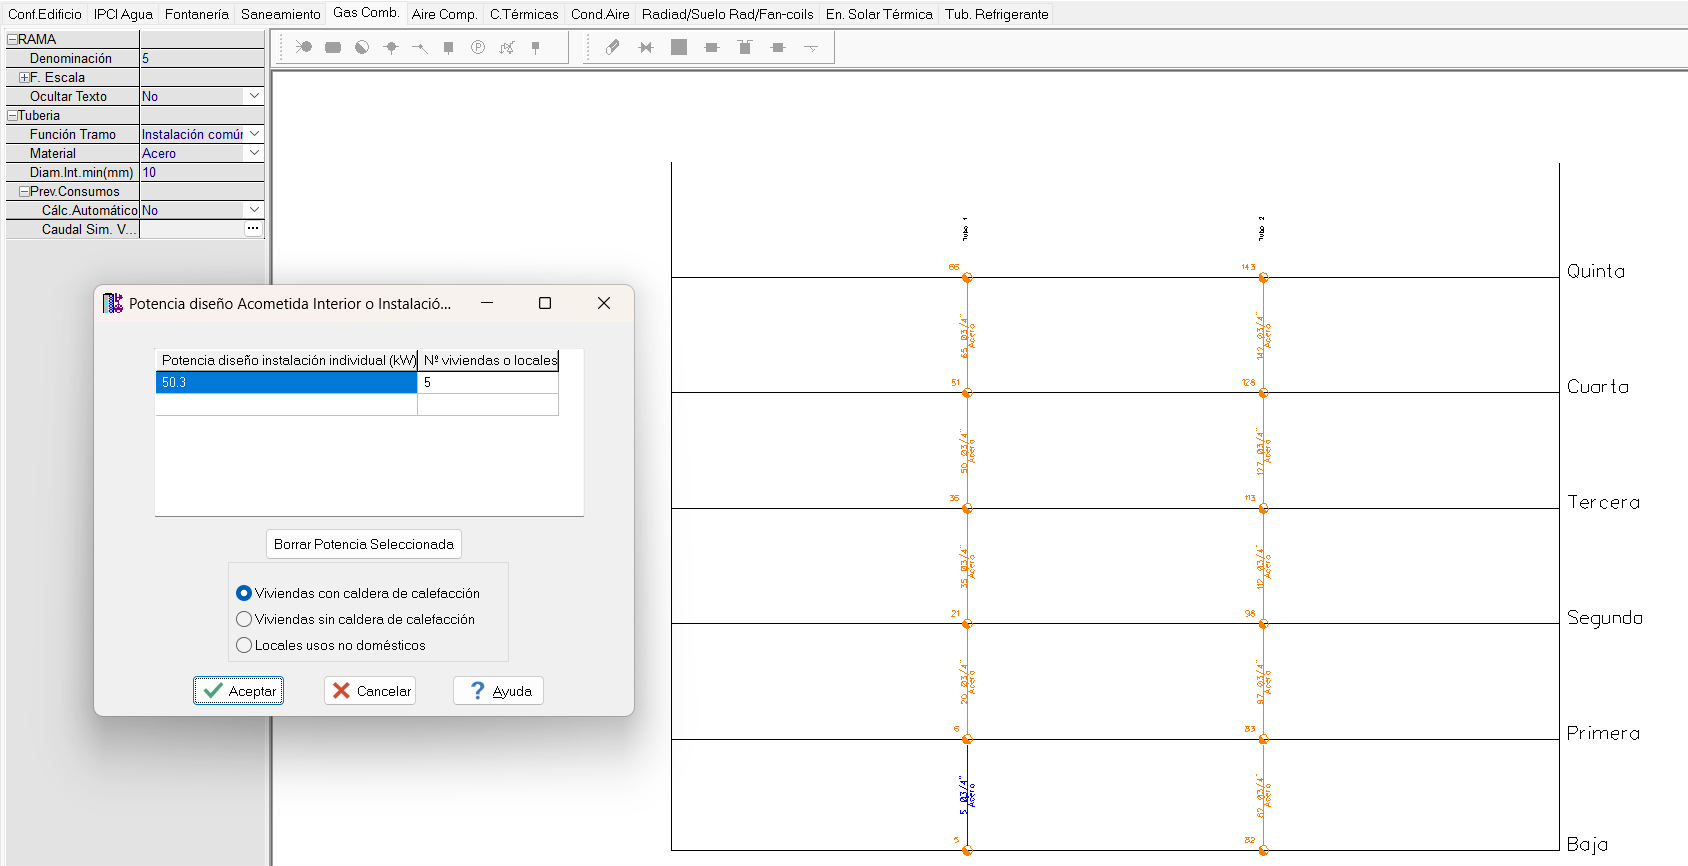
\includegraphics[width = 0.78\textwidth]{Figuras/asignacion_potencias-vivienda.png}
	\caption{Asignación de potencia de diseño y número de viviendas para el cálculo automático de simultaneidad en el programa. Fuente: Elaboración grupal.}
	\label{fig:asignacion_potencias_vivienda}
\end{figure}

\subsection{Topología del edificio y selección del esquema de instalación}

El edificio se modela como un bloque plurifamiliar de cinco plantas y dos viviendas por planta. Esta repetición permite definir una planta tipo y propagar su esquema en altura. En el programa, la configuración gráfica del edificio permite crear los niveles, asignar las cotas de cada planta y vincular los planos de fondo que sirven como referencia para trazar la red. En edificios con plantas iguales, el manual empleado permite trabajar con una planta representativa siempre que los tramos comunes incorporen la previsión de consumos total aguas abajo, evitando que el cálculo considere únicamente las viviendas dibujadas \cite{DMElectManual}.

La definición de plantas empleada en el modelo se muestra en \cref{fig:definicion_plantas}. Esta figura actúa como transición entre el plano arquitectónico y el modelo hidráulico: fija la lectura de niveles, alturas y repetición vertical que posteriormente condiciona la longitud de los montantes y la identificación de los puntos más desfavorables.

\begin{figure}[H]
	\centering
	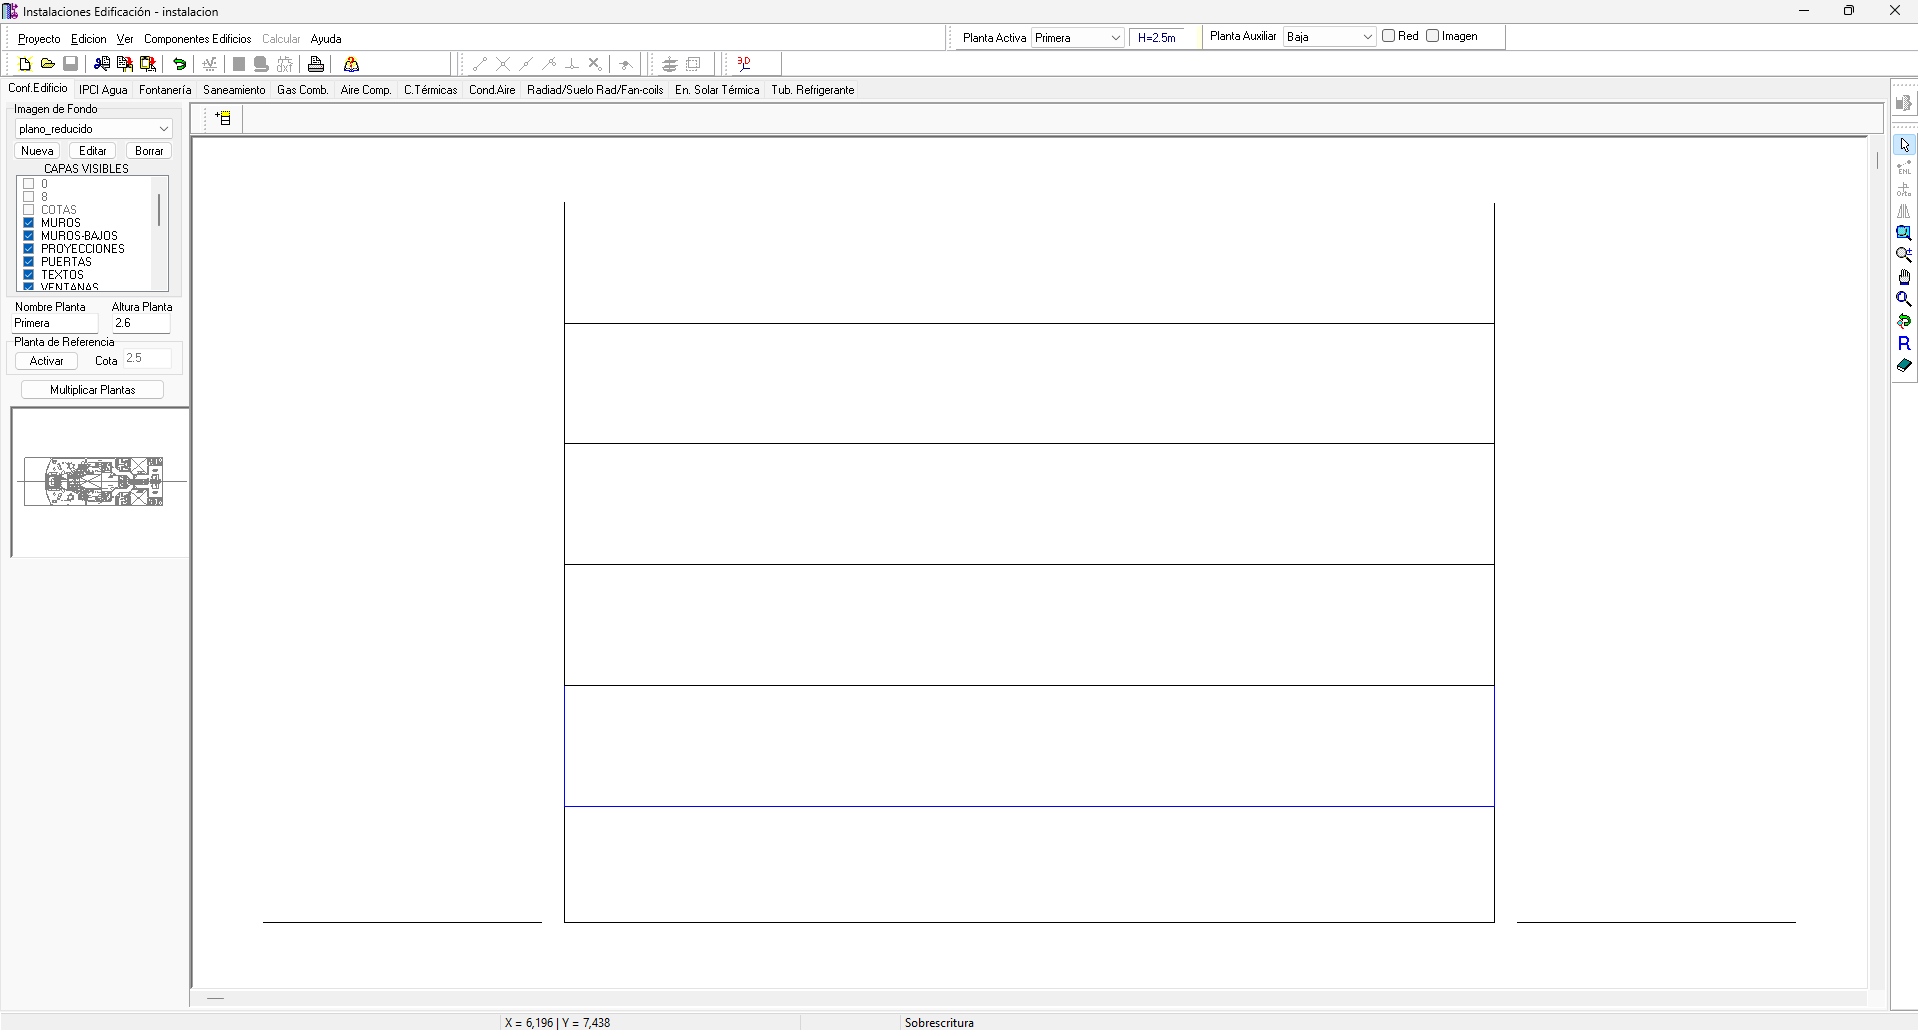
\includegraphics[width =\textwidth]{Figuras/definicion_plantas.png}
	\caption{Definición de las plantas. Fuente: Elaboración grupal.}
	\label{fig:definicion_plantas}
\end{figure}

La solución adoptada separa la instalación en una parte común y en derivaciones individuales. La acometida conecta la red de distribución con la llave de acometida; a partir de esta frontera funcional se desarrolla la acometida interior, la zona de contadores, los montantes que alimentan las diez viviendas del edificio y las derivaciones hasta la cocina. La instalación individual comienza aguas abajo del contador o de la llave de vivienda y termina en las llaves de conexión de cada aparato. Esta división responde a la repetición de plantas y viviendas, y también define responsabilidades de corte, mantenimiento y comprobación, tal como recogen la terminología y los criterios de diseño de la UNE 60670 \cite{UNE60670_2_2023,UNE60670_4_2023}.

\begin{figure}[H]
	\centering
	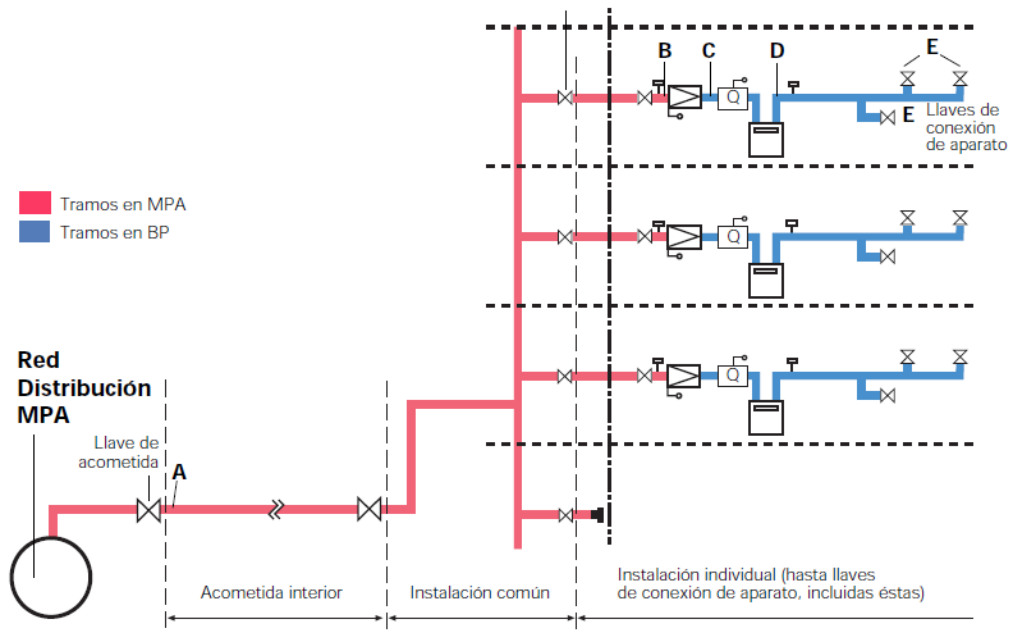
\includegraphics[width = 0.75\textwidth]{Figuras/esquema_instalacion.png}
	\caption{Modelo de instalación seleccionada. Fuente: Proporcionada por el tutor.}
	\label{fig:esquema_instalacion}
\end{figure}

El esquema de \cref{fig:esquema_instalacion} representa esta decisión de diseño. La instalación común agrupa los tramos que transportan caudal simultáneo hacia varias viviendas, mientras que las instalaciones individuales atienden los aparatos de cada vivienda. Este planteamiento permite que los diámetros sean mayores en las zonas de acumulación de demanda y decrezcan hacia los receptores, reduciendo material sin perder presión disponible.

\subsection{Justificación del trazado elegido}

El trazado elegido responde al carácter libre indicado en el guion de la práctica. Se ha optado por un recorrido claro desde la acometida hasta la centralización o ubicación de contadores, los montantes y las derivaciones interiores hasta la cocina, donde se concentran los aparatos de utilización. Esta organización facilita la lectura del esquema y evita recorridos innecesarios en el interior de las viviendas.

La repetición de dos viviendas por planta permite resolver la red con una lógica modular: los montantes distribuyen el suministro en altura y las derivaciones de cada vivienda repiten un patrón semejante. Con ello se obtiene una alimentación ordenada, se reducen cambios de dirección y longitudes superfluas, y se mantiene una correspondencia directa entre el plano, el esquema vertical y el anejo de cálculo. Esta solución también simplifica la interpretación de los puntos críticos que el programa marca tras el cálculo.

\subsection{Equipos instalados y materiales de la instalación}

Los equipos principales se han incorporado al modelo por su función hidráulica, de regulación, medición y corte:

\begin{itemize}
	\item Acometida y llave de acometida, como punto de entrada desde la red de distribución y corte general de la instalación.
	\item Contadores, para registrar el consumo de cada suministro y representar la pérdida de carga asociada a la medición.
	\item Reguladores o reductores de presión, para pasar de la presión disponible en la red común a la presión de utilización de las viviendas.
	\item Válvulas de corte, para sectorizar la instalación común y permitir intervenciones localizadas.
	\item Llaves de vivienda, para delimitar y aislar cada instalación individual.
	\item Llaves de conexión de aparato, para permitir la intervención sobre cada receptor sin dejar fuera de servicio el resto de la vivienda.
\end{itemize}

Los purgadores se entienden únicamente como accesorios previstos por el guion dentro del conjunto de elementos necesarios para la instalación, sin desarrollarse como operación o resultado del proyecto. El limitador de caudal no se incorpora al modelo porque no resulta necesario para el esquema desarrollado y porque el módulo disponible no lo incluye como accesorio modelable dentro de la red calculada.

Los contadores introducen una pérdida de carga propia y, por tanto, no son elementos neutros desde el punto de vista del cálculo. Su posición debe ser compatible con la accesibilidad y ventilación del recinto, especialmente en centralizaciones, donde la UNE 60670-5 exige aberturas de ventilación superior e inferior y reserva del recinto para instalaciones de gas \cite{UNE60670_5_2023}. En el modelo de cálculo, el programa incorpora estos componentes en la cadena de pérdidas desde la acometida hasta los aparatos.

En cuanto a materiales, el proyecto combina acero en los tramos de mayor caudal y materiales como cobre o multicapa P/Al/PEX en derivaciones e instalaciones interiores, de acuerdo con las familias admitidas por la UNE 60670-3. El acero se ajusta a los tramos comunes y montantes por su rigidez y disponibilidad en diámetros normalizados; el cobre y los sistemas multicapa facilitan la ejecución de recorridos interiores de menor caudal. En todos los casos, las uniones deben ser compatibles con el material elegido y con la presión de operación, aplicando soldadura fuerte o uniones mecánicas certificadas cuando corresponda \cite{UNE60670_3_2023}.

Los aparatos considerados son caldera, cocina o encimera, horno y secadora. Su papel en el cálculo no se limita a la potencia nominal: cada equipo exige una presión mínima de entrada, ventilación adecuada según su tipo y una llave de conexión accesible. La ventilación de locales con aparatos de circuito abierto debe dimensionarse de acuerdo con los criterios aplicables de la UNE 60670-6, considerando el consumo calorífico de los aparatos instalados y los mínimos reglamentarios para uso doméstico \cite{UNE60670_6_2023}.

\subsection{Optimización del dimensionamiento}

El cálculo se ha realizado en modo de diseño. En el modelo se definen la topología, los materiales, los aparatos, la presión de suministro, la potencia de diseño de las instalaciones individuales y el número de viviendas servidas por los tramos comunes. A partir de esos datos, el programa calcula caudales simultáneos, selecciona diámetros normalizados y resuelve las pérdidas de carga tramo a tramo. En los tramos de baja presión utiliza una formulación lineal de Renouard, mientras que en media presión trabaja con la diferencia cuadrática de presiones; ambas expresiones aparecen recogidas en el anejo de cálculo exportado.

La relación básica entre potencia y caudal procede de la potencia de diseño y del poder calorífico superior:

\begin{equation}
	Q = \frac{P}{PCS}
\end{equation}

donde $Q$ es el caudal volumétrico, $P$ la potencia de diseño y $PCS$ el poder calorífico superior del gas. Esta relación explica la base física del cálculo, pero la asignación de consumos simultáneos se realiza dentro del programa al configurar la potencia de diseño y las viviendas servidas. La memoria conserva la trazabilidad del método y remite al anejo para el detalle completo de fórmulas, ramas y nudos \cite{UNE60670_4_2023,DMElectManual}.

El programa no sustituye el criterio técnico de revisión. Aunque automatiza el cálculo y marca los elementos críticos, los resultados deben interpretarse, las advertencias deben comprobarse y los datos de partida deben contrastarse con el alcance del proyecto. La optimización se ha centrado en revisar diámetros, velocidades, pérdidas de carga y presión en el receptor más desfavorable. En este proyecto se adoptaron como restricciones principales una velocidad máxima de \SI{20}{\meter\per\second}, pérdidas secundarias del \SI{20}{\percent}, presión relativa mínima de aparato de \SI{180}{mmca}, pérdida máxima de \SI{25}{mmca} en baja presión y pérdida máxima de \SI{500}{mmca} en media o alta presión, valores reflejados en el anejo de cálculo.

Una vez calculada la red, el programa identifica la rama de mayor velocidad y el nudo de menor presión dinámica mediante un asterisco. La ausencia de errores de presión o velocidad no se interpreta de forma aislada; se contrasta con los valores numéricos del anejo, con el mapa de estados y con las exigencias de presión mínima de aparato y velocidad máxima de la UNE 60670-4 \cite{UNE60670_4_2023,DMElectManual}.

\section{Resultados y discusión}

\subsection{Análisis de la verificación hidráulica mediante mapa de estados}

El mapa de estados generado por el programa resume la validez hidráulica de la instalación. Los elementos que incumplen límites de presión, pérdida de carga o velocidad se marcan como errores o advertencias, mientras que los puntos críticos de la instalación calculada aparecen destacados para facilitar su revisión. En este proyecto, la comprobación se centra en dos resultados: la acometida, por concentrar el mayor caudal simultáneo y la mayor velocidad, y el aparato de utilización más desfavorable, por representar el extremo donde la presión disponible es menor.

\begin{figure}[H]
	\centering
	\begin{subfigure}[b]{0.12\textwidth}
		\centering
		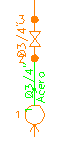
\includegraphics[width=\textwidth]{Figuras/acometida_desfavorable.png}
	\end{subfigure}
	\hfill
	\begin{subfigure}[b]{0.7\textwidth}
		\centering
		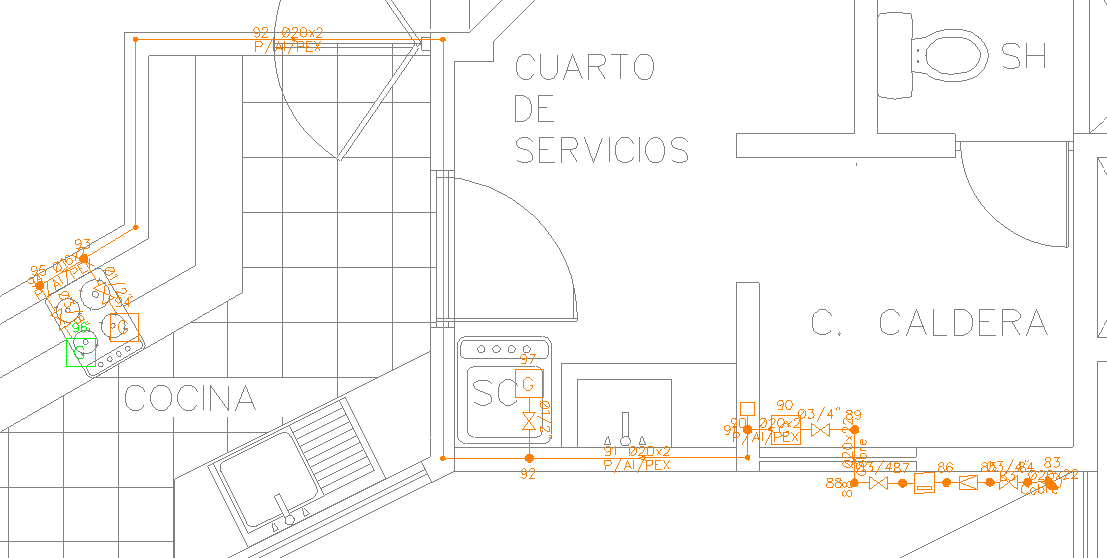
\includegraphics[width=\textwidth]{Figuras/aparato_utilizacion_desfavorable.png}
	\end{subfigure}
	\caption{Puntos más desfavorables. (a) Acometida (b) Horno (Vivienda 1, planta 1). Fuente: Elaboración grupal.}
	\label{fig:puntos_desfavorables}
\end{figure}

La rama de acometida presenta la mayor velocidad de la red, un resultado coherente con su función de tramo común que centraliza el caudal total de simultaneidad de la instalación. Al concentrar la demanda acumulada de todas las viviendas antes de la distribución por montantes, este tramo se configura como el más exigente desde el punto de vista cinético. No obstante, la velocidad obtenida (\SI{15,4}{\meter\per\second}) cumple con el límite de \SI{20}{\meter\per\second} fijado por la normativa UNE 60670-4.

La presión de regulación o suministro de la acometida se fija en \SI{1500}{mmca}. Este valor sitúa el tramo inicial en Media Presión A y queda dentro del intervalo de trabajo previsto para alimentar la instalación común y los montantes antes de la regulación de las instalaciones individuales. En el avance por la instalación común se producen pérdidas de carga pequeñas frente a la presión disponible, hasta llegar a los reguladores y contadores. Tras la regulación, las viviendas trabajan en baja presión, con valores próximos a \SI{250}{mmca} antes de distribuirse hacia los receptores. Esta reducción controlada es coherente con el anejo de cálculo y con las presiones finales obtenidas en los aparatos.

\subsection{Análisis de los puntos singulares más desfavorables}

El punto de menor presión dinámica identificado por el programa es el aparato de cocina-horno del nudo 96, situado en la vivienda 1 de la planta 1 según la documentación gráfica generada. El anejo le asigna una presión relativa de \SI{228}{mmca}, un caudal de \SI{1,2}{\cubic\meter\per\hour} y una potencia de \SI{12}{\kilo\watt}. Este valor supera la presión mínima de aparato considerada en el cálculo, \SI{180}{mmca}, por lo que el punto más desfavorable mantiene margen de funcionamiento.

La lectura técnica del resultado es que, si el receptor con menor presión cumple, los restantes aparatos quedan en una situación igual o más favorable. Las calderas presentan presiones en torno a \SI{244}{mmca}; las secadoras, alrededor de \SI{241}{mmca}; y las encimeras, en torno a \SI{230}{mmca}. La diferencia entre estos valores refleja la combinación de longitud de recorrido, diámetro disponible, caudal de diseño y pérdidas en accesorios. No se observa una caída brusca incompatible con el esquema: las pérdidas se reparten de manera progresiva desde la acometida hasta cada instalación individual.

La coherencia del dimensionamiento también se aprecia en la distribución de diámetros. Los tramos de acometida, acometida interior y montantes transportan caudales simultáneos elevados y conservan diámetros de acero DN 20. En las derivaciones individuales se emplean diámetros menores, ajustados al caudal de cada grupo de aparatos. Esta reducción progresiva evita sobredimensionar toda la red, pero mantiene la presión mínima en el receptor más desfavorable. El diseño resultante equilibra seguridad, continuidad de suministro y economía de material.

Los planos incluidos en \cref{anex:planos} documentan el trazado en planta, la acometida, la instalación común, los montantes y el esquema vertical. El anejo de \cref{anex:calculos} conserva la trazabilidad completa del cálculo: fórmulas aplicadas, hipótesis generales, tabla de ramas, tabla de nudos, presiones, caudales, velocidades y diámetros. La memoria se apoya en esos documentos para no duplicar tablas extensas en el cuerpo principal.

\section{Conclusiones}

El diseño de la instalación receptora de gas natural queda justificado para el edificio plurifamiliar analizado. La metodología aplicada, basada en el modelado de la red en el programa, ha permitido resolver el trazado libre solicitado desde la acometida en MPA hasta las cocinas de las viviendas, incorporando los equipos necesarios de regulación, medición y corte.

Se confirma que la red proyectada cumple las restricciones de velocidad, pérdida de carga y presión mínima adoptadas en el cálculo. La acometida concentra la mayor velocidad de la instalación y el aparato más desfavorable conserva presión suficiente, por lo que los resultados principales del programa son coherentes con el dimensionamiento obtenido.

La optimización se ha realizado ajustando diámetros y revisando velocidades, pérdidas de carga y presión en el receptor más desfavorable, sin duplicar en la memoria las tablas extensas del anejo. El resultado mantiene diámetros mayores en los tramos comunes, donde se acumula la demanda simultánea calculada por el programa, y reduce progresivamente las secciones hacia las instalaciones individuales.

Finalmente, la realización de este proyecto ha permitido aplicar de forma práctica los conceptos teóricos vistos en clase. El proceso de diseño, desde el planteamiento del trazado hasta la resolución mediante una herramienta profesional de cálculo, ha reforzado la comprensión de la jerarquización de redes, la simultaneidad de consumos y la influencia de la presión disponible en el funcionamiento de los aparatos.

%%%% Referencias------------------------

\cleardoublepage
\phantomsection
\addcontentsline{toc}{section}{Bibliografía}
\printbibliography[title={Bibliografía}]


\myappendix{Planos}
\label{anex:planos}

\includepdf[pages=-, fitpaper=true]{Figuras/planta_distribucion.pdf}
\includepdf[pages=-, fitpaper=true]{Figuras/acometida_ins_individual.pdf}
\includepdf[pages=-, fitpaper=true]{Figuras/instalacion_comun-montantes.pdf}
\includepdf[pages=-, fitpaper=true]{Figuras/esquema_vertical.pdf}

\myappendix{Cálculos}
\label{anex:calculos}

\includepdf[pages=-]{Figuras/Anejo_calculo.pdf}


\end{document}
